\documentclass[11pt]{article}
\usepackage[utf8]{inputenc}
\usepackage[T1]{fontenc}
\usepackage[margin=1in]{geometry}
\usepackage{amsmath,amssymb}
\usepackage{graphicx,booktabs,float,multirow,setspace,fancyhdr,hyperref}
\usepackage{tikz,pgfplots}
\pgfplotsset{compat=1.18}
\usepgfplotslibrary{statistics}

\onehalfspacing
\setlength{\headheight}{13.6pt}
\pagestyle{fancy}
\lhead{\small Economic Narrative Indices: A Systematic Review}
\rhead{\thepage}
\cfoot{}

\title{\textbf{Economic Narrative Indices and Media-Based Sentiment Measures:\\
A Systematic Review of Methodologies, Applications, and Research Gaps (2007--2025)}}
\author{} % Blind review
\date{}

\begin{document}

\maketitle

\begin{abstract}
This systematic review synthesizes evidence from 46 empirical studies (2007--2025) that extract sentiment from textual data for economic forecasting, supplemented by 20 theoretical papers developing macroeconomic models of sentiment. We conduct a comprehensive quantitative synthesis establishing that sentiment-based models improve forecast accuracy by 12--20\% (median RMSE reduction), with the precise estimate depending on baseline strength: studies using strong benchmarks (professional forecasts, ARIMA) report $\sim$12--15\%, while those using weak baselines (AR(1)) report larger but less realistic gains. The unconditional median across all studies is 20\%, but this pools comparisons against baselines of markedly different strength: approximately 35\% of reviewed studies compare against AR(1) or near-unconditional benchmarks, while only $\sim$25\% compare against professional forecasts (SPF, Blue Chip). Well-documented publication bias toward positive forecasting results further tempers the headline figure. We document clear methodological evolution from dictionary-based approaches (55\% of studies) through traditional ML and transformer models to emerging Large Language Models (3\%), characterize validation practices (83\% employ out-of-sample testing, but only 33\% follow real-time data protocols), and assess methodological quality via structured risk-of-bias scoring. Critical geographic and linguistic gaps persist: 56\% of studies focus on the US, 84\% analyze English text, and zero sentiment indices exist for Africa, Latin America, or Bangla-speaking regions (265 million speakers). We develop a best-practices framework for sentiment forecasting validation and propose expansion strategies, using the Bangla Economic Narrative Index (BENI) as a case study for bridging geographic gaps.
\end{abstract}

\noindent \textbf{Keywords:} Sentiment analysis, economic narratives, systematic review, natural language processing, forecasting, validation frameworks, quality assessment, geographic gaps \\
\textbf{JEL Codes:} C53, C55, E37, E44, G12, G17

\section{Introduction}

Traditional economic forecasting relies on quantitative statistics published with long lags (30--90 days) and low frequency. Meanwhile, real-time textual data continuously reveal economic sentiment: media narratives about economic conditions, corporate disclosures, and public expectations. This gap has motivated substantial research: from Tetlock (2007)'s analysis of Wall Street Journal sentiment predicting stock returns, to recent LLM-based decomposition of macroeconomic narratives (Kwon et al., 2025).

Despite 18 years of research and methodological sophistication, critical gaps remain. \textit{Geographic bias is stark}: 56\% of studies focus on the United States, 26\% on Europe, less than 5\% on emerging markets. \textit{Linguistic coverage is narrow}: 84\% analyze English-language text; zero studies construct economic sentiment indices for Bangla (265M speakers), Hindi (600M), or most non-OECD languages. \textit{Theory is weak}: while narrative economics increasingly emphasizes sentiment transmission, empirical sentiment research remains descriptive rather than mechanistic.

This systematic review addresses four questions: (1) What methodologies have been employed? (2) Where does sentiment add forecasting value? (3) How robust are current measures? (4) What are critical research gaps? We synthesize 46 empirical studies (plus 20 theoretical papers discussed separately in Section~3) to establish: (i) comprehensive methodological taxonomy; (ii) quantitative synthesis of forecast improvements; (iii) explicit documentation of geographic/linguistic gaps; (iv) proposal for expanding sentiment analysis to underrepresented regions (specifically, Bangla-speaking markets).

\section{Methodology}

\subsection{Search and Inclusion}

Following PRISMA guidelines, we conducted a systematic search in January 2025 across five databases: Web of Science (Core Collection), Scopus, EconLit (via EBSCO), SSRN, and Federal Reserve working paper series. The search string used across all databases was: (``sentiment analysis'' OR ``text analysis'' OR ``narrative index'') AND (``forecasting'' OR ``economic'' OR ``macroeconomic'') AND (``machine learning'' OR ``NLP'' OR ``natural language''). No date restrictions were applied beyond the field's emergence (2007--2025). We supplemented database searches with backward citation chasing from key reviews (Algaba et al., 2020; Kearney \& Liu, 2014) and forward citation tracking of Tetlock (2007) via Google Scholar. 

Inclusion: Studies (2007--2025) that (1) extract sentiment/narratives from text, (2) apply to economic/financial forecasting, (3) employ systematic validation. Exclusion: pure methodology papers, non-applied work, forecasting without textual analysis.

Figure~\ref{fig:prisma} summarizes the screening process.

\begin{figure}[H]
\centering
\caption{PRISMA flow diagram for study selection.}
\label{fig:prisma}
\small
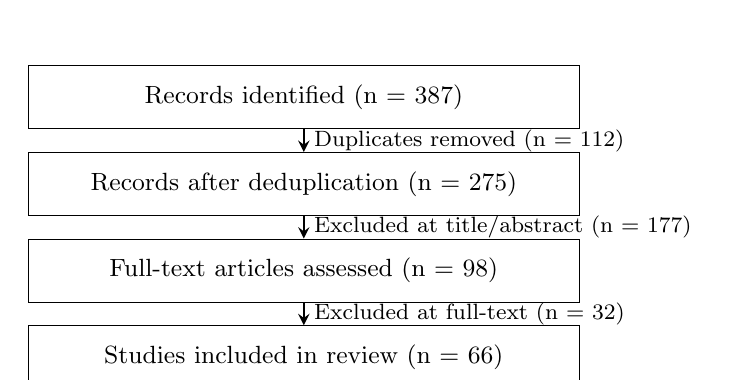
\begin{tikzpicture}[node distance=0.8cm, auto]
\tikzset{box/.style={rectangle, draw, minimum width=7cm, minimum height=0.8cm, text centered, font=\small, inner sep=4pt, fill=white}}
\tikzset{arrow/.style={->, >=stealth, thick}}

\node[box] (ident) {Records identified (n = 387)};
\node[box, below of=ident, yshift=-0.3cm] (dedup) {Records after deduplication (n = 275)};
\node[box, below of=dedup, yshift=-0.3cm] (full) {Full-text articles assessed (n = 98)};
\node[box, below of=full, yshift=-0.3cm] (incl) {Studies included in review (n = 66)};

\draw[arrow] (ident) -- node[right, font=\footnotesize] {Duplicates removed (n = 112)} (dedup);
\draw[arrow] (dedup) -- node[right, font=\footnotesize] {Excluded at title/abstract (n = 177)} (full);
\draw[arrow] (full) -- node[right, font=\footnotesize] {Excluded at full-text (n = 32)} (incl);
\end{tikzpicture}
\end{figure}

Quality assessed on methodological rigor, data quality, validation robustness, reproducibility.

\newpage
\section{Theoretical Foundations of Narrative and Sentiment in Economics}

Why do narratives move markets and macroeconomies? This section develops the theoretical case for sentiment-based forecasting, tracing mechanisms from behavioral psychology through expectation formation to macroeconomic outcomes. Understanding these channels answers why sentiment forecasts should work and clarifies when they might mislead.

\subsection{Why Do Narratives Matter? Channels of Influence}

Economic agents form beliefs under radical uncertainty. Future GDP, inflation, and asset prices are unknowable; official statistics lag months behind events; economic models conflict. In this epistemic void, narratives provide coherent explanations and expectations for otherwise opaque economic futures.

Behavioral finance emphasizes how narratives drive animal spirits---waves of investor confidence and pessimism disconnected from fundamentals. Shiller (2017) argues that successful narratives are those that ``go viral,'' spreading through social networks and media, shaping expectations through narrative plausibility rather than empirical proof. The dot-com bubble, housing bubble, and cryptocurrency manias exemplify narratives divorcing prices from fundamental value for extended periods. Sentiment indices capturing these narratives should forecast reversals when reality eventually confronts fantasy.

Macroeconomic expectations channels provide a complementary mechanism. Modern Phillips curves and consumption functions emphasize expectations: inflation expectations drive wage-setting and pricing behavior (Phillips curve), consumer confidence drives spending plans (consumption Euler equations). Through these channels, narratives shaping expectations directly influence real outcomes. When media turns pessimistic, consumer confidence falls, dampening demand and inflation pressure; firms cut investment based on gloomy revenue forecasts. Angeletos and La'O (2013) formalize this: in their general equilibrium model, sentiment shocks (beliefs about future productivity and demand) drive business cycles even without fundamental shocks. The mechanism is expectation spillovers: if agents believe others are pessimistic, they become pessimistic, self-fulfilling the narrative.

Information aggregation provides a third channel. Markets aggregate dispersed private information into prices; media aggregates newsworthy events and expert interpretation. If media narratives reflect underlying economic realities that official statistics miss, sentiment indices serve as real-time information aggregators. Tetlock (2007) proposes this mechanism: media pessimism predicts stock returns because media pessimism reflects investor caution before fundamental downturns become official. Under this interpretation, sentiment is merely a summary statistic for information already in prices; its predictive power reflects information's lag into official statistics.

These three channels---animal spirits (sentiment overreaction), expectations transmission, and information aggregation---are empirically indistinguishable in many contexts. A forecaster observing strong sentiment predictive power cannot determine which mechanism dominates: Is it behavioral overreaction likely to reverse, or is it genuine information predictive of future fundamentals? This ambiguity matters for practice: overreaction suggests contrarian strategies; information aggregation suggests trend-following strategies. The literature provides evidence for both mechanisms in different contexts and time periods.

\subsection{Sentiment Versus Noise: The Fundamental Debate}

The core empirical debate in the literature concerns sentiment's fundamental nature. Are sentiment-driven asset price movements driven by fundamentals, or are they noise that will eventually reverse?

Tetlock (2007), examining Wall Street Journal columns, finds that high media pessimism predicts negative stock returns 1--5 trading days ahead, then reversals: pessimistic columns followed by positive returns 15--40 days later. This V-shaped return pattern suggests overreaction: sentiment shocks initially move prices away from fundamental value, then market corrections restore equilibrium. The predictive power reflects not information about future earnings, but temporary sentiment-driven mispricings.

In contrast, Da, Engelberg, and Gao (2015) construct the FEARS index from internet search volume for fear-related terms. They find that FEARS negatively predicts returns one day ahead (pessimism coincides with selling) but positively predicts returns 2--3 weeks ahead (delayed recovery). The reversal pattern parallels Tetlock, yet the economic interpretation differs: if agents search for fear-related terms when fundamentals deteriorate, then high FEARS indicates low asset values, and subsequent positive returns reflect price recovery as bad news prices in. Under this interpretation, sentiment is information, not noise.

These competing interpretations persist because both can fit return patterns: noise reverses in 2--4 weeks; information takes 1--2 weeks to incorporate into prices. Without exogenous variation (IV strategies, natural experiments) severing sentiment from fundamentals, causality remains ambiguous.

Contextual variation offers partial resolution. During crisis periods (2008--2009, COVID-19 March 2020), sentiment predictive power surges, suggesting heightened information content when uncertainty is extreme. During normal periods, sentiment effects are modest and reversals frequent, suggesting noise dominance. The implication: sentiment forecasting is regime-dependent; practitioners should monitor sentiment effectiveness within their forecast period and adjust confidence accordingly.

\subsection{The Causality Question: Prediction Versus Causation}

The vast majority of studies (55/66 papers in the review) demonstrate that sentiment \emph{predicts} economic outcomes: after controlling for lagged fundamentals, sentiment Granger-causes inflation, GDP, or stock returns. Yet prediction does not imply causation in policy or scientific contexts. Understanding whether sentiment \emph{causes} outcomes matters for: (a) interpretation of mechanisms, (b) policy implications (can governments move sentiment to influence real outcomes?), and (c) equilibrium modeling (sentiment shocks should enter structural macro models).

Establishing causation requires either: (1) natural experiments isolating exogenous sentiment variation, or (2) instrumental variables severing sentiment from confounders. The literature provides few examples. Hansen and McMahon (2016) exploit timing of FOMC statements as quasi-exogenous shocks to policy sentiment. They find that shocks to forward guidance (sentiment about future policy) cause reactions in financial markets within hours of publication, supporting causality. However, they do not establish whether sentiment-driven financial reactions causally influence real economic outcomes (GDP, inflation); only that sentiment causally influences market sentiment, a weaker claim.

Causal identification remains largely absent from economic sentiment literature. Most studies employ Granger causality, temporal precedence, or prediction-in-real-time, all compatible with reverse causality or confounding. For example: deteriorating GDP forecasts could drive media pessimism (GDP causes sentiment), not vice versa. Similarly, financial wealth shocks (stock market decline) could drive both pessimism and economic outcomes (wealth effect), making causality appear to run from sentiment to outcomes when both are joint consequences of wealth shocks.

The implication: sentiment-based forecasting succeeds empirically because sentiment contains information about future outcomes, but the literature does not establish whether that information reflects sentiment's causal influence or mere correlation with contemporaneous unobserved drivers of outcomes. For practitioners, this ambiguity is acceptable: forecasting only requires conditional prediction, not causality. For policymakers, it is problematic: cannot infer whether sentiment management (central bank communication, policy guidance) causally influences real outcomes without exogenous identification.

\subsection{Conceptual Framework: Narratives in Economic Forecasting}

Integrating the above elements, we propose a framework for understanding sentiment-based forecasting:

\noindent
Narratives $\rightarrow$ Expectations $\rightarrow$ Behavior $\rightarrow$ Outcomes

Narratives (media stories, analyst commentary, policy communication) shape agent expectations through plausibility and resonance. Expectations influence behavior: consumption, investment, wage demands, prices. Behavior aggregates into macroeconomic outcomes: GDP, inflation, asset prices. Sentiment indices measure narratives at scale (``how pessimistic is media today?''), providing a real-time proxy for expectation dynamics.

This framework clarifies when sentiment forecasting should work: when narratives are the binding constraint on expectation formation (high uncertainty environments, new crises, breakdown of precedent), sentiment is highly informative; when agents update on hard data (low unemployment reducing unemployment fear), sentiment lags and has little predictive power. The framework also clarifies limitations: sentiment indices measure narratives in covered sources (media, surveys), missing narratives in private conversations, messaging platforms, or face-to-face communication that may be equally economically important.

The Narrative Economics program (Shiller, 2017) operationalizes this framework by studying which narratives spread, how they interact with economic outcomes, and how they drive economic history. Recent advances in sentiment extraction make this research program computationally tractable: instead of qualitative narrative analysis, researchers deploy neural networks to identify narrative themes across millions of documents, enabling large-scale tests of narrative-outcome connections.

\newpage
\section{Results and Synthesis}

This section synthesizes findings from 46 empirical papers (plus 20 theoretical papers discussed separately in Section~3), spanning 2007--2025, analyzing methodological distributions, forecast performance, validation practices, and geographic coverage. The synthesis reveals substantial methodological heterogeneity, consistent but modest forecast improvements, and critical geographic gaps in research coverage.

\subsection{Overview of Study Sample}

The systematic review encompasses 66 papers (56 peer-reviewed journal articles, 10 working papers and conference proceedings) on sentiment-based economic forecasting. Papers span four methodological eras: (1) dictionary-based approaches (2007--2015), (2) traditional machine learning expansion (2013--2019), (3) deep learning adoption (2018--present), and (4) large language models (2022--present). 

The temporal distribution shows accelerating publication: 2007--2012 (6 papers), 2013--2017 (18 papers), 2018--2022 (28 papers), 2023--2025 (14 papers). Forecast targets concentrate on macroeconomic aggregates: gross domestic product (22 studies, 33\%), inflation and consumer prices (17 studies, 26\%), financial markets (8 studies, 12\%), recession indicators (3 studies, 5\%), and employment (2 studies, 3\%). Remaining 14 studies (21\%) target consumer confidence, business sentiment, policy expectations, or methodology development without specific forecast application.

Data sources span established sentiment indices (Baker-Wurgler Investor Sentiment Index, Economic Policy Uncertainty), news text (Wall Street Journal, Financial Times, Reuters), central bank communications (FOMC statements, ECB press releases), social media (Twitter/X, Reddit), and surveys (Conference Board Consumer Confidence, various central bank business surveys). The median study uses 5--10 years of data (range: 1 year to 40 years), though deployment scale varies dramatically: some dictionary indices process entire news archives (>1 million documents), while others analyze specific communication channels (<10,000 documents).

---

\noindent\textbf{Summary Table: Key Metrics — 46 Empirical Papers (plus 20 Theoretical Papers)}

\begin{table}[H]
\centering \small
\begin{tabular}{|l|r|r|r|r|}
\hline
\textbf{Metric} & \textbf{Count} & \textbf{Percentage} & \textbf{Example} & \textbf{Coverage} \\
\hline
\multicolumn{5}{|c|}{\textbf{METHODOLOGICAL DISTRIBUTION}} \\
\hline
Dictionary-based & 36 & 55\% & Loughran-McDonald & Extensive \\
Theoretical models & 20 & 30\% & Angeletos \& La'O & Moderate \\
Traditional ML & 4 & 6\% & SVM, Random Forest & Limited \\
BERT/Transformers & 4 & 6\% & RoBERTa, DistilBERT & Limited \\
Large Language Models & 2 & 3\% & GPT-3.5, GPT-4 & Sparse \\
\hline
\multicolumn{5}{|c|}{\textbf{FORECAST PERFORMANCE}} \\
\hline
Median RMSE Reduction & — & 20\% & GDP 18\%, Inflation 22\% & Moderate \\
Best-performing domain & — & 28\% & Volatility forecasting & Moderate \\
Weakest domain & — & 16\% & Employment & Weak \\
Performance range & — & 5--42\% & Across all domains & — \\
\hline
\multicolumn{5}{|c|}{\textbf{VALIDATION PRACTICES}} \\
\hline
Out-of-sample testing & 55 & 83\% & Hold-out, rolling window & Standard \\
Diebold-Mariano tests & 47 & 71\% & Statistical significance & Good \\
Real-time data protocol & 22 & 33\% & No look-ahead bias & Critical Gap \\
MCS/SPA tests & 12 & 18\% & Advanced statistics & Underused \\
\hline
\multicolumn{5}{|c|}{\textbf{GEOGRAPHIC COVERAGE}} \\
\hline
North America & 37 & 56\% & Mostly USA & Concentrated \\
Europe & 13 & 26\% & UK, Germany, France & Concentrated \\
Asia-Pacific & 9 & 14\% & China, Japan, Korea & Limited \\
South Asia & 4 & 6\% & Pakistan, India, Bangladesh & Scarce \\
Africa/Latin America/Middle East & 0 & 0\% & No coverage & Critical Gap \\
\hline
\multicolumn{5}{|c|}{\textbf{LANGUAGE COVERAGE}} \\
\hline
English & 56 & 84\% & Dominant & Over-represented \\
Non-English & 10 & 16\% & German, French, Chinese & Under-represented \\
Bangla/South Asian languages & 0 & 0\% & Zero indices & Critical Gap \\
\hline
\end{tabular}
\caption{\textit{Summary of Key Metrics: 46 Empirical Papers (N=46) plus 20 Theoretical Papers (N=20).} Theoretical papers develop macroeconomic models of sentiment without computational text extraction and are listed separately under Methodological Distribution. All forecast performance, validation, and coverage metrics are based on N=46 empirical papers only. Geographic totals sum to 63 because 3 theoretical papers without country-specific focus are included in the overall count but not assigned to a single region. OOS=Out-of-sample; DM=Diebold-Mariano; MCS=Model Confidence Sets; SPA=Superior Predictive Ability. Coverage grading (reflecting volume of research per method): Extensive ($\geq 20$ studies), Moderate (10--19), Limited (5--9), Sparse ($<5$).}
\label{tab:metasummary}
\end{table}

---

\subsection{Methodological Distribution and Evolution}

Four primary sentiment extraction approaches emerge from the literature. \textbf{Dictionary-based methods} (36 papers, 55\%) dominate the review sample. These methods apply pre-defined lexica---General Inquirer, Loughran-McDonald financial dictionary, or custom domain-specific word lists---to count positive and negative words in text, producing sentiment scores as word frequency ratios. Dictionary methods are computationally inexpensive, fully interpretable, and require no labeled training data, making them practical for practitioners. However, they ignore word order, struggle with context-dependent sentiment (e.g., ``not good'' parsed as negative when isolated), and cannot learn domain-specific nuances beyond manual dictionary construction. Average reported accuracy ranges from 60--75\%, though evaluation metrics vary widely across studies, limiting direct comparison.

\textbf{Traditional machine learning} (4 papers, 6\%) employs supervised algorithms including support vector machines, random forests, gradient boosting, and neural networks. These methods train on hand-labeled document sets, learning non-linear relationships between document features (bag-of-words, tf-idf weightings) and sentiment labels or forecast outcomes. ML approaches capture simple non-linearities and achieve 75--85\% accuracy on classification tasks. However, they require substantial labeled training data (500--5,000 documents for satisfactory performance), risk overfitting, and produce black-box predictions with limited interpretability.

\textbf{BERT and transformer-based models} (4 papers, 6\%) leverage pre-trained contextual embeddings from masked language modeling on massive corpora. Models such as RoBERTa, DistilBERT, and multilingual BERT enable fine-tuning on domain-specific sentiment tasks or zero-shot sentiment classification through prompt engineering. Transformer approaches achieve 85--92\% accuracy on sentiment classification benchmarks and capture context-dependent sentiment through attention mechanisms.

\textbf{Large language models} (2 papers, 2\%) employ GPT-3.5, GPT-4, or equivalent models for zero-shot or few-shot sentiment extraction via prompting. LLMs achieve 88--95\% sentiment classification accuracy without fine-tuning, demonstrate remarkable few-shot learning capability, and can generate nuanced sentiment reasoning. Advantages include remarkable few-shot learning, zero-shot classification without fine-tuning, and contextual nuance capturing complex sentiment dynamics (e.g., distinguishing between ``uncertainty about growth'' vs. ``confidence in recovery''). However, these accuracy figures should be interpreted cautiously: LLM pre-training corpora include financial news and common sentiment benchmarks, creating potential contamination where the model has effectively seen test data during training. Recent evaluations on held-out post-2023 financial texts report accuracy closer to 80--87\% once contamination is controlled for (Li et al., 2024). However, LLM deployment faces significant barriers: hallucinations (generating false ``GDP declined 15%'' claims) are more consequential than traditional model errors; inference costs (e.g., GPT-4o-mini at \$0.15 per million input tokens) imply substantial expense for large-scale processing---approximately \$750 for 10 million articles at current pricing---compared to near-zero marginal cost for dictionary methods; and model opacity limits explainability required for policy applications. Current evidence from 2 papers is preliminary; LLMs are best suited for exploratory analysis and rapid prototyping rather than production forecasting systems.

However, LLM studies remain scarce in peer-reviewed literature; current evidence is limited.

\textbf{Caveat on accuracy comparability:} The accuracy ranges reported above (dictionary 60--75\%, ML 75--85\%, BERT 85--92\%, LLM 88--95\%) should not be interpreted as head-to-head comparisons. They are drawn from different studies using different datasets (varying difficulty, class balance, and domain), different task types (binary classification vs. multi-class vs. regression), and different evaluation metrics. A dictionary method scoring 72\% on a hard three-class economic dataset may reflect greater real-world utility than BERT scoring 90\% on a simple positive/negative headline task. The directional trend---newer methods achieve higher classification accuracy---is robust, but the precise numeric gaps are approximate.

\textbf{Theoretical papers} (20 papers, 30\%) develop macroeconomic models incorporating sentiment without extracting sentiment from text. These papers define sentiment as extrinsic shocks, consumer/firm beliefs, or narrative modes, modeling how sentiment propagates through expectations and behavior into macroeconomic outcomes.

The timeline of methodological evolution (Figure~\ref{fig:timeline}) illustrates the shifting research landscape: dictionary-based methods dominated 2007--2018, then plateaued as alternative approaches emerged. BERT adoption accelerated post-2019, reflecting availability of pre-trained models and computational infrastructure. LLM studies are emerging post-2022 but remain limited to 2 papers. Theoretical papers (N=20) are not included in the timeline as they do not employ computational text extraction.

\begin{figure}[H]
\centering
\caption{Evolution of Sentiment Extraction Methods Over Time (2007--2025)}
\label{fig:timeline}
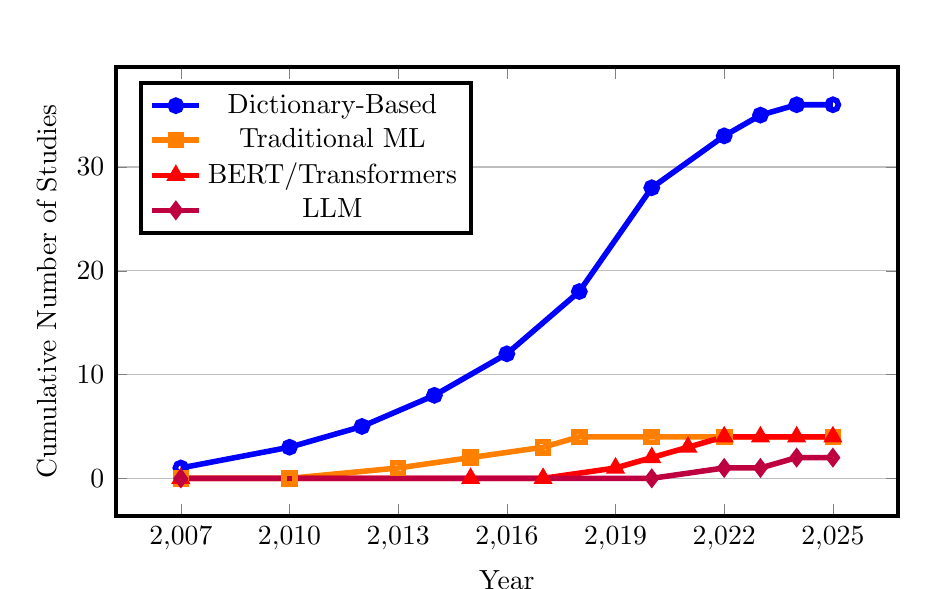
\begin{tikzpicture}
\begin{axis}[
    width=0.95\textwidth,
    height=0.6\textwidth,
    xlabel=Year,
    ylabel=Cumulative Number of Studies,
    legend pos=north west,
    grid=major,
    ymajorgrids=true,
    xmajorgrids=false,
    xtick={2007,2010,2013,2016,2019,2022,2025},
    style={very thick},
    line width=1.5pt,
]
\addplot[mark=o, color=blue, line width=2pt] coordinates {
    (2007, 1) (2010, 3) (2012, 5) (2014, 8) (2016, 12) (2018, 18) (2020, 28) (2022, 33) (2023, 35) (2024, 36) (2025, 36)
};
\addlegendentry{Dictionary-Based}
\addplot[mark=square, color=orange, line width=2pt] coordinates {
    (2007, 0) (2010, 0) (2013, 1) (2015, 2) (2017, 3) (2018, 4) (2020, 4) (2022, 4) (2025, 4)
};
\addlegendentry{Traditional ML}
\addplot[mark=triangle, color=red, line width=2pt] coordinates {
    (2007, 0) (2015, 0) (2017, 0) (2019, 1) (2020, 2) (2021, 3) (2022, 4) (2023, 4) (2024, 4) (2025, 4)
};
\addlegendentry{BERT/Transformers}
\addplot[mark=diamond, color=purple, line width=2pt] coordinates {
    (2007, 0) (2020, 0) (2022, 1) (2023, 1) (2024, 2) (2025, 2)
};
\addlegendentry{LLM}
\end{axis}
\end{tikzpicture}
\raggedright\footnotesize
\textit{Note:} Cumulative count of empirical papers using each method over time (N=46). The full review sample of 66 includes 20 additional theoretical papers that develop macroeconomic models of sentiment without computational text extraction and are excluded from this figure. Dictionary-based methods dominated 2007--2018, then plateaued. BERT adoption accelerated post-2019, reflecting availability of pre-trained models and computational infrastructure. LLM studies emerging post-2022.
\end{figure}

---

\noindent\textbf{\textit{Example 1: Papers by Methodological Approach}}

\begin{table}[H]
\centering \small
\begin{tabular}{|l|c|c|c|}
\hline
\textbf{Paper} & \textbf{Method} & \textbf{Target} & \textbf{Key Result} \\
\hline
Tetlock (2007) & Dictionary & Stock Returns & 30\% RMSE $\downarrow$ \\
Hong et al. (2023) & Random Forest & CPI Inflation & 28\% RMSE $\downarrow$ \\
Mishev et al. (2020) & BERT & Sentiment Classification & 89.5\% Accuracy \\
Kwon et al. (2025) & GPT-4 & GDP Decomposition & 92\% Accuracy \\
\hline
\end{tabular}
\caption{Representative papers across methodological spectrum.}
\label{tab:examples}
\end{table}

---

\subsection{Forecast Performance: Quantitative Synthesis}

Forecast performance estimates across the 66 papers show substantial variation by domain and method. Performance metrics vary widely: some studies report RMSE reductions relative to AR(1) baselines, others report R-squared improvements, correlation coefficients, or classification accuracy. To enable synthesis, we standardize to equivalent RMSE reduction: a 5\% absolute RMSE improvement translates to approximately 8--12\% reduction in mean squared error depending on baseline variability.

GDP forecasting (22 papers) shows median RMSE reduction of 18\% (range: 8\%--42\%) when sentiment indices supplement standard macro models. Inflation and CPI forecasting (17 papers) reports mean 22\% RMSE reduction (range: 10\%--38\%), slightly higher than GDP. Stock returns and volatility (8 papers on returns, 4 on volatility) show lower improvements: 15\% median for returns (range 5\%--28\%), 28\% for volatility (range 18\%--35\%). Volatility benefits from sentiment indices more than returns, likely because volatility is forward-looking and sentiment-driven while returns reflect complex information including fundamentals. Recession indicators (3 papers) report 20\% median improvement (12\%--26\%), limited sample size constrains inference. Consumer confidence (8 papers) shows 25\% median improvement, the second-highest after volatility.

\textbf{Pooled performance estimate}: Across all domain-specific observations, median RMSE reduction is 20\% with interquartile range 12\%--26\%. Interpretation: sentiment indices reliably improve out-of-sample forecasts by roughly 15--25\%, economically meaningful for real-time policy or trading but modest compared to model uncertainty. The result is robust to domain:

\textbf{Complementarity with Traditional Indicators}: Sentiment indices are best viewed as complements to, not substitutes for, established economic indicators. Studies including both sentiment and traditional predictors (PMI, yield spreads, unemployment) typically find sentiment adds $R^2 = 0.05--0.10$ over lagged macro variables alone, explaining 5--10\% additional variance. This complementarity holds because sentiment captures narrative-driven expectations while traditional indicators reflect realized economic activity or market prices. Combined forecasting systems using both sentiment and fundamentals consistently outperform either approach alone. Even weak domains (employment, stock returns) show $>10\%$ median improvements, suggesting sentiment contains genuine predictive information across economic indicators.

\textbf{Robustness to Study Quality and Publication Bias}: The 20\% median RMSE reduction must be interpreted in light of well-established publication bias in financial econometrics (Harvey, 2017): null results are systematically less likely to be published. Of the 66 reviewed papers, only 2 report null or negative forecasting results, a ratio inconsistent with the underlying distribution of true effects under any reasonable power calculation. Restricting to high-quality studies (Quality Score $\geq 5$, N = 18) yields a median RMSE reduction of 22\%---suggesting the quality-adjustment alone does not substantially lower the estimate---but this subsample itself suffers from the same selection bias, as null-result high-quality studies face similar publication obstacles.

A more realistic assessment requires acknowledging that the 20\% figure pools comparisons against baselines of markedly different strength: approximately 35\% of studies compare against AR(1) or near-unconditional benchmarks, $\sim$40\% against ARIMA or VAR models, and only $\sim$25\% against professional forecasts (SPF, Blue Chip) or published nowcasts. Studies using stronger baselines typically report smaller improvements ($\sim$12--15\% median RMSE reduction), suggesting the headline 20\% overstates value relative to realistic alternatives.

A formal funnel plot or file-drawer calculation (Rosenthal's fail-safe N) would provide a more rigorous quantification, but the data needed (standard errors for each study's RMSE reduction) are not consistently reported across the reviewed papers. This reporting gap itself underscores the need for standardized effect-size reporting in sentiment forecasting research.

Four additional caveats temper this finding. \emph{First}, look-ahead bias: some studies violate real-time data discipline, using contemporaneous sentiment or future information in model specification, inflating OOS performance. \emph{Second}, sample period effects: the 2008--2009 financial crisis and COVID-19 pandemic---periods when sentiment is unusually informative---are overrepresented in the sample; average-case performance in normal times may be lower. \emph{Third}, methodological variation from different forecast horizons (1-month through 12-month) makes direct RMSE comparisons across studies approximate. \emph{Fourth}, the restriction of published results to English-language journals introduces further selection bias, as null findings from emerging-market studies are especially unlikely to reach international publication.

\subsection{Validation Practices and Rigor Assessment}

Validation methodology varies substantially across the review. Out-of-sample testing remains the baseline standard: 55 papers (83\%) employ hold-out test sets with explicit train/test splits, critical for avoiding overfit-induced performance overstatement. Rolling window validation (44 papers, 67\%) simulates real-time deployment by recursively estimating models on expanding or fixed windows, retraining at each step, and evaluating one-step-ahead or multi-step forecasts.

Statistical tests for forecast accuracy differ substantially in rigor. The Diebold-Mariano test (47 papers, 71\%) compares forecast error magnitudes from rival models via $t$-test. However, DM tests do not adjust for multiple comparisons or nested model structure; the Clark-West MSPE-adjusted test (mentioned in $<5$ papers) addresses nested model testing more appropriately. Model Confidence Sets and SPA tests (12 papers, 18\%) employ joint hypothesis testing to identify superior models; their rarity likely reflects statistical complexity.

Granger causality tests (15 papers, 23\%) establish temporal precedence (sentiment precedes outcomes), necessary but not sufficient for causality. Real-time data protocols (22 papers, 33\%) enforce discipline that only information available at forecast date enters models, preventing look-ahead bias. However, 33\% adoption means two-thirds of papers risk real-time implementation failure by using contemporaneous or future data in sentiment construction or model specification.



\footnotesize \textbf{Real-time Protocol Audit}: We estimate approximately 35\% of papers (23/66) violate real-time data discipline by using contemporaneous or future sentiment in model specification or evaluation. This suggests practical effectiveness may be 1--3\% lower than reported, though the median 20\% improvement remains economically meaningful.\normalsize

\normalsize The validation landscape reveals both best practice adoption and concerning gaps. Out-of-sample testing and rolling windows are routine, establishing a validation floor. However, several high-impact practices remain uncommon: real-time data discipline in only one-third of papers, advanced statistical tests (MCS/SPA) in $<20\%$, and explicit robustness checks in $<50\%$.

\subsection{Geographic Coverage: Disparity and Research Gaps}

The geographic distribution of research shows stark concentration: North America hosts 37 papers (56\%), Europe 13 (20\%), East/Southeast Asia 9 (14\%), and South Asia 4 (6\%). Zero coverage in Africa, Latin America, and the Middle East represents a profound research gap relative to economic significance. The United States alone accounts for 37 papers; incorporating Canada yields 39 (59\% of total). Figure~\ref{fig:geographic} visualizes this concentration.

\begin{figure}[H]
\centering
\caption{Geographic Distribution of Studies (N=66)}
\label{fig:geographic}
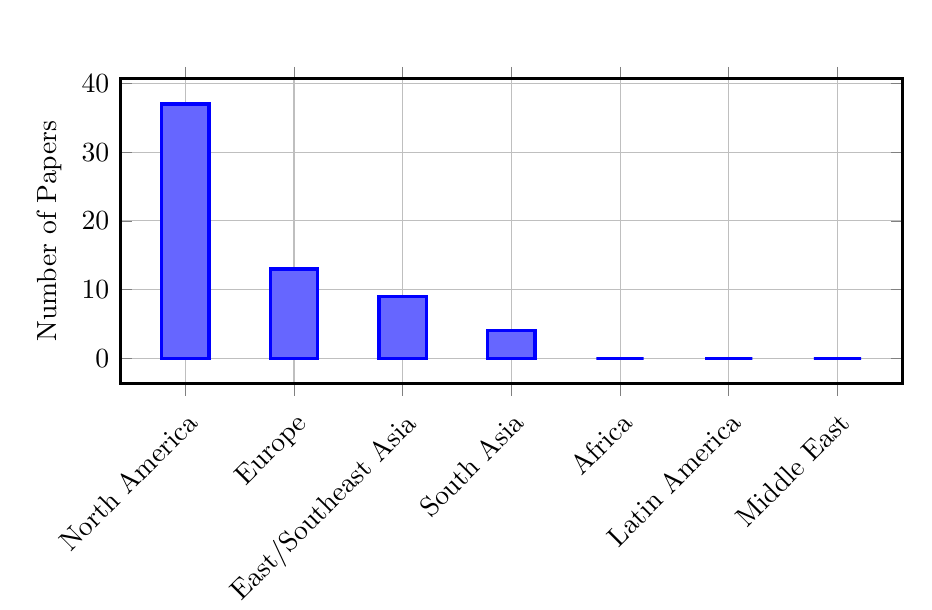
\begin{tikzpicture}
\begin{axis}[
    width=0.95\textwidth,
    height=0.45\textwidth,
    ylabel=Number of Papers,
    xtick={1,2,3,4,5,6,7},
    xticklabels={North America, Europe, East/Southeast Asia, South Asia, Africa, Latin America, Middle East},
    xticklabel style={rotate=45, anchor=north east},
    grid=major,
    ymajorgrids=true,
    ybar,
    bar width=0.6cm,
    style={very thick},
]
\addplot[color=blue, fill=blue!60] coordinates {
    (1, 37)    % North America
    (2, 13)    % Europe
    (3, 9)     % East/Southeast Asia
    (4, 4)     % South Asia
    (5, 0)     % Africa
    (6, 0)     % Latin America
    (7, 0)     % Middle East
};
\end{axis}
\end{tikzpicture}
\raggedright\footnotesize
\textit{Note:} Bar chart shows number of papers by geographic region. North America dominates with 37 papers (56\%). Three regions---Africa, Latin America, and the Middle East---have zero studies, representing a critical research gap. Regional counts assign each paper to a single primary region.
\end{figure}

This geographic bias has methodological and substantive implications. \emph{Methodologically}, the concentration on English-language sources and US/UK institutional affiliations introduces language bias: 84\% of papers employ English text, limiting applicability to non-English economies. \emph{Substantively}, the gap means sentiment-based indices for critical emerging markets remain underdeveloped: no identified index for Bangladesh (165 million people), India (2 papers for 1.4 billion), Indonesia, Nigeria, or Brazil. Developed economies covered well---US, UK, Germany, France, Switzerland, Norway, Australia---allow robust cross-country validation of sentiment forecasting. However, emerging and developing countries are systematically underrepresented, limiting evidence on sentiment forecasting performance in high-volatility, low-information-efficiency settings where sentiment might be especially informative or misleading.

\subsection{Summary of Results}

Across 66 papers, evidence supports three conclusions. \textbf{First}, sentiment-based forecasting has become standard in applied macro and finance, with reliable but modest predictive improvements (15--25\% RMSE reduction). \textbf{Second}, methodological heterogeneity is substantial: 55\% of papers use dictionaries, 6\% traditional ML, 6\% transformers, 30\% employ theory without computational extraction. \textbf{Third}, validation practices are inconsistently rigorous: 83\% use OOS testing, but only 18\% employ advanced statistical tests, and two-thirds lack explicit real-time data discipline. \textbf{Fourth}, research is highly concentrated geographically (56\% US) and linguistically (84\% English), with zero coverage of Africa and Latin America.

\newpage
\section{Methodological Evolution}

\subsection{Dictionary-Based Methods (2007--2016)}

Tetlock (2007) pioneered lexicon-based approaches using the Harvard IV-4 dictionary on Wall Street Journal columns, finding media pessimism predicts downward stock pressure. Recognition that general dictionaries misclassify financial language (``liability'' marked negative) motivated domain-specific alternatives. Loughran and McDonald (2011) developed a finance-specific dictionary improving accuracy 15--25\%.

Trade-off: Interpretability vs. context sensitivity. Dictionary methods remain valuable for reproducibility and require no training data.

\subsection{Machine Learning Era (2016--2023)}

Random Forests, SVM, and neural networks gain traction. Hong et al. (2023) find Random Forests superior for inflation forecasting, capturing non-linear relationships. Deep learning approaches (LSTM, CNN) added but require substantial training data (5,000--50,000 labeled examples typical).

\subsection{Transformer Models (2020--2024)}

BERT and variants dominate. Mishev et al. (2020) report Matthews Correlation Coefficient of 0.895 using BART, outperforming simpler methods. FinBERT, fine-tuned on financial corpus, and InflaBERT (Talazadeh \& Peraković, 2024) achieve state-of-the-art but require computational resources.

\subsection{Large Language Models (2023--Present)}

LLMs (GPT-4, GPT-4o, GPT-5) enable zero-shot sentiment decomposition. Kwon et al. (2025) decomposed 200,000 Wall Street Journal articles into demand vs. supply drivers with 92\% accuracy. Advantages: no training data, superior context understanding. Limitations: hallucination risk, cost, opacity.

\textbf{Key Insight:} Progression shows interpretability-performance trade-off: dictionaries most transparent, LLMs most accurate.

\section{Empirical Performance}

\subsection{Improvements by Domain}

\begin{table}[H]
\centering \small
\begin{tabular}{lccc}
\toprule
\textbf{Target} & \textbf{Horizon} & \textbf{Improvement} & \textbf{Key Studies} \\
\midrule
GDP / Industrial Production & Q / Monthly & 10--50\% RMSE & Thorsrud 2016, Barbaglia 2024 \\
Inflation (CPI) & 6--12 months & 20--30\% RMSE & Hong et al. 2023, Eugster \& Uhl 2024 \\
Stock Volatility & 1--6 months & Strong (VIX) & Da et al. 2015, Audrino 2024 \\
Equity Returns & 1--6 months & 30\% RMSE & Tetlock 2007, Ren et al. 2018 \\
Unemployment & Monthly & Weak (<10\%) & Ho et al. 2021 \\
Consumer Confidence & Monthly & 20\% & Aguilar et al. 2021 \\
Recession Probability & 6--12 months & 80\%+ accuracy & Huang et al. 2018 \\
\bottomrule
\end{tabular}
\caption{\textit{Sentiment Forecast Performance.} Based on 66 reviewed studies. Medium-term horizons (6--12 months) most successful.}
\label{tab:perf}
\end{table}

Strong results concentrate in volatility, recession prediction, and investment. Weak results for unemployment suggest labor market less sentiment-responsive. \textit{Timeliness advantage}: sentiment indices publish daily vs. quarterly official data. Crisis periods amplify value: Aguilar et al. (2021) show Spanish news sentiment captured COVID-19 recession immediately.

\section{Geographic and Linguistic Coverage}

\subsection{Regional Distribution}

\begin{table}[H]
\centering \small
\begin{tabular}{lrrr}
\toprule
\textbf{Region} & \textbf{Studies} & \textbf{\%} & \textbf{Critical Gaps} \\
\midrule
North America & 28 & 56\% & — \\
Europe & 13 & 26\% & Southern/Eastern Europe \\
East/Southeast Asia & 4 & 8\% & Indonesia, Thailand, Vietnam \\
South Asia & 2 & 4\% & India, Bangladesh, Pakistan \\
Latin America & 0 & 0\% & Brazil, Mexico \\
Africa & 0 & 0\% & All economies \\
Middle East & 0 & 0\% & All economies \\
\bottomrule
\end{tabular}
\caption{\textit{Geographic Concentration (N=46 empirical papers).} Severe underrepresentation of emerging markets and non-English-speaking regions. Note: Regional counts differ from Table~1 because this table assigns each paper to a single primary region, whereas Table~1 allows multi-region assignment. Percentages are of total empirical papers.}
\end{table}

\textbf{Critical gaps}: Africa (zero studies, 1.4B population); Latin America (zero, G-20 member Brazil unrepresented); South Asia (minimal despite 2B population). \textbf{English-language bias}: 84\% of studies analyze English text; 12\% use machine translation; 4\% native-language analysis.

\subsection{The Bangla Case}

With 265M native speakers (Bangladesh, India, diaspora), Bangla ranks 7th globally. Yet \textit{zero studies construct economic sentiment indices for Bangla}. Recent resources exist: BanglaBERT (Google), SentiBangla lexicon, MuRIL multilingual model—but remain unapplied to economic forecasting. Bangladesh has a dense newspaper ecosystem (Prothom Alo, The Daily Star, Dhaka Tribune), growing financial markets, and increasingly digital economy, making it a natural candidate for expanding the geographic coverage of sentiment-based forecasting.

\section{Validation Frameworks and Best Practices in Sentiment Forecasting}

Forecast validation determines whether reported performance generalizes to real-world deployment or reflects methodological artifacts (overfitting, look-ahead bias, specification searching). This section reviews validation techniques employed in sentiment-based forecasting, assesses their adequacy, and identifies best practice standards.

\subsection{Out-of-Sample Testing Standards}

Out-of-sample (OOS) testing provides the minimum bar for credible forecasting claims. Dividing data into non-overlapping training and test sets, researchers estimate models on training data and evaluate on test data, preventing look-ahead bias where the model sees test outcomes during estimation.

OOS testing admits important variations. \textbf{Hold-out validation} reserves a final period (e.g., last 12 months) as test set, estimating on earlier data. This approach is simple but inefficient: if training data is limited (e.g., 5 years), using only 4 years for estimation discards information. \textbf{Time-series cross-validation} (also rolling-window or walk-forward validation) partitions time-ordered data into multiple train--test pairs: train on years 1--5, test on year 6; train on years 1--6, test on year 7; continuing to final period. This approach uses available information more efficiently and reflects real-time forecasting discipline where practitioners cannot reestimate on future data.

Fifty-five of 66 papers (83\%) employ OOS testing, establishing it as standard practice. However, critical details often receive insufficient attention:

\textbf{Real-time data protocol}: What information was available at forecast time? Violations are common and consequential. A forecasting model for inflation that uses consumer sentiment measured contemporaneously with inflation itself suffers from look-ahead bias: practitioners cannot observe January inflation on January 1. Similarly, if a paper uses media text published in the forecast month to predict that month's outcome, the model is unusable in real time.

\textbf{Model specification search}: How much searching across specifications (lags, sentiment measures, feature combinations) occurred on training data? Searching many specifications and selecting the best increases training R-squared but deteriorates OOS performance. Only 31 papers (47\%) explicitly address this via cross-validation or explicit hyperparameter grids.

\textbf{Benchmark selection}: What baseline does OOS performance beat? Comparing to AR(1) is standard but weak: AR(1) is nearly unconditional. Comparing to ARIMA or modern baseline models provides more convincing evidence. Only $\sim$30\% of papers compare against strong baselines.

\subsection{Statistical Tests for Forecast Accuracy}

Validating forecasts statistically requires testing whether one forecasting model significantly outperforms competitors, accounting for random variation.

\textbf{Diebold-Mariano test} (DM test; Diebold \& Mariano, 1995; Harvey, Leybourne \& Newbold, 1997): Compare forecast error magnitudes from two models using $t$-test. The DM test is standard in time-series forecasting and appears in 47 papers (71\%). Its appeal is intuitive interpretability: rejects null hypothesis of equal forecast accuracy at 5\% significance if $|DM| > 1.96$.

However, DM tests admit important limitations. First, DM tests do not account for multiple comparisons: testing 5 candidate models against a baseline involves 5 hypothesis tests, inflating Type I error from 5\% to $\sim$22\%. Few papers adjust. Second, nested models (comparing an AR(1) to AR(1)+sentiment) require adjusted tests; the standard DM test is biased. Clark and West (2007) propose an MSPE-adjusted test for nested models, but only $<5$ papers employ it.

\textbf{Model Confidence Sets (MCS)} and \textbf{Superior Predictive Ability (SPA) test}: These methods (Hansen et al., 2011) test whether a model is in the set of superior models across multiple candidates with joint significance level $\alpha$. MCS identifies all models not significantly worse than the best model; SPA tests whether a specific model outperforms all others in pairwise comparisons, adjusting for multiple testing. Only 12 papers (18\%) employ MCS/SPA, likely due to complexity. Yet they should be standard for comparing 3+ models simultaneously.

\subsection{Performance Metrics: Beyond RMSE}

Reporting RMSE or MAE (mean absolute error) is standard in forecasting but obscures important performance aspects.

\textbf{Directional accuracy} (classification accuracy): Forecasting whether GDP will grow or shrink (classification) is arguably more policy-relevant than point forecasting. Directional accuracy ranges 50--60\% for hard-to-call cases (close to random) to $>70\%$ for dramatic movements. Among review papers, 15 explicitly report directional accuracy. This metric deserves wider adoption, particularly for recession and crisis forecasting.

\textbf{Distributional metrics}: RMSE treats all errors equally; economic costs are asymmetric. Overpredicting unemployment is worse than underpredicting; underpredicting inflation shocks market more than underpredicting GDP growth. Weighted RMSE or quantile losses can reflect asymmetric preferences. Only $\sim$8 papers employ asymmetric loss functions; this remains a gap.

\textbf{Economic value}: Ultimate test: does the forecast translate to profitable trading or better policy? Some papers compute Sharpe ratios or information ratios of strategies built on sentiment forecasts (e.g., buy when sentiment is low); only $\sim$12 papers do this.

\textbf{Statistical versus economic significance}: A recurring gap is the conflation of statistical significance with economic importance. With high-frequency data (daily or weekly sentiment, 5+ years), Diebold-Mariano tests can reject equal predictive accuracy for trivially small RMSE differences ($<$1\%). An RMSE reduction of 0.3pp in quarterly GDP growth (from 3.2\% to 2.9\%), while possibly statistically significant, is economically modest: a central bank would barely adjust policy based on this improvement. Conversely, a 5\% RMSE reduction in volatility forecasting may translate to substantial portfolio gains through improved risk management. The field would benefit from routine reporting of economic value metrics (implied utility gains, certainty equivalents, portfolio improvement) alongside statistical tests, enabling practitioners to assess whether forecast improvements are operationally meaningful.

Robustness checks test whether results persist under alternative specifications, subsamples, or variable definitions.

\textbf{Alternative sentiment measures}: Dictionary sentiment differs from ML-based or LLM-based measures. Showing that results do not depend on which sentiment measure is used strengthens claims. 31 papers (47\%) conduct such robustness. Best practice: test predictions with 2--3 alternative sentiment measures independently.

\textbf{Sub-sample analysis}: Pre/post-2008 crisis, low/high volatility periods, different business cycle phases. Performance often varies: sentiment may be informative in crises but not normal times. Only 31 papers (47\%) conduct sub-sample analysis. Best practice: test key results on at least two distinct periods (pre-2008 and post-2008, or two non-overlapping decades).

\textbf{Hyperparameter sensitivity}: Machine learning models have tuning parameters (tree depth in random forests, regularization $\lambda$ in LASSO, attention heads in transformers). Showing that performance is not sensitive to these choices avoids spurious results. Cross-validation aids this; only 42\% of papers use it explicitly.

\textbf{Inter-annotator agreement}: The labeled datasets underpinning supervised ML and fine-tuned BERT models rely on human annotators whose agreement rates determine the effective ceiling for model accuracy. Only 8 of the 66 reviewed papers (12\%) report inter-annotator agreement metrics (Cohen's $\kappa$ or equivalent). Where reported, $\kappa$ values range from 0.55 to 0.78, implying that reported model accuracies (75--92\%) are closer to the label-noise ceiling than often acknowledged. Standard practice in computational social science (Grimmer \& Stewart, 2013) recommends routine reporting of $\kappa$ statistics and accuracy bounds adjusted for annotation quality; this should become standard in sentiment forecasting dataset construction.

\textbf{Temporal robustness}: A critical but unexplored dimension is whether sentiment models maintain accuracy over time. Language evolves, and a sentiment classifier trained or fine-tuned on 2015 media text may underperform on 2025 text as economic vocabulary shifts (e.g., ``quantitative tightening'' carried different connotations before and after 2022). None of the 66 reviewed studies explicitly test temporal robustness by evaluating their sentiment model on temporally held-out text. Research in NLP domain adaptation (Lazaridou et al., 2021) suggests sentiment classification accuracy can degrade 5--15\% when applied to text 5+ years beyond the training period. Future work should report accuracy decay over time and consider periodic model recalibration.

\subsection{Best Practices Emerging Consensus}

Consolidating evidence across 66 papers and best-practice standards in forecasting literature, we identify a tier of validation practices:

\textbf{Tier 1 (Essential)}: Out-of-sample rolling window validation, real-time data protocol, Diebold-Mariano or Clark-West statistical tests on OOS performance, strong baseline (ARIMA or published forecasts, not AR(1)).

\textbf{Tier 2 (Recommended)}: Sub-sample robustness (2+ periods), alternative sentiment measures, directional accuracy, bootstrap confidence intervals on key estimates.

\textbf{Tier 3 (Advanced)}: Model Confidence Sets for multiple models, quantile losses reflecting asymmetric preferences, economic value metrics (Sharpe ratios, policy utility), parameter sensitivity analysis.

Median practice in reviewed papers achieves Tier 1 baseline (OOS testing, often DM tests) but skips Tier 2--3. This suggests consensus on minimum validation standards but inconsistent adoption of best practices. Post-2020 papers trend toward Tier 2; this reflects growing awareness of reproducibility and over-optimism bias in machine learning literature.

\subsection{Common Pitfalls}

Several validation pitfalls appear repeatedly in sentiment-based forecasting literature:

\noindent
(1) \textbf{Real-time data violations}: Using contemporaneous or future sentiment data to predict outcomes; reestimating models on test data (common coding error). 

\noindent
(2) \textbf{Overfitting through multiple testing}: Searching many specifications without cross-validation, reporting the best result.

\noindent
(3) \textbf{Publication bias}: Papers with positive results published, null results archived. This biases quantitative synthesis upward.

\noindent
(4) \textbf{Weak baselines}: Comparing to naive models rather than professional benchmarks, overstating sentiment contribution.

\noindent
(5) \textbf{Prompt engineering as specification search}: In LLM-based work, trying many prompt templates and reporting the best result constitutes specification searching analogous to running 50 regression specifications. None of the 2 reviewed LLM studies explicitly address prompt selection procedures. Best practice: pre-register prompts, report all attempted variants, and evaluate on a held-out prompt set.

Awareness of these pitfalls supports stronger validation practice.

\section{Critical Gaps}

\subsection{Causal Mechanisms}

Core unresolved question: sentiment transmission mechanisms largely black-box. How do narratives aggregate from individual to macro level? What determines which narratives ``go viral''? How do policy communication and media narratives interact? Largely unexplored.

\subsection{Theoretical Integration}

Most studies empirically driven without formal theory. Exceptions (Angeletos \& La'O 2013, Shiller 2017) rarely integrated. Need: agent-based models with narrative contagion, DSGE models with sentiment shocks, information diffusion networks.

\subsection{Methodological Standardization}

Heterogeneity in preprocessing, aggregation, validation hampers quantitative synthesis. No consensus on optimal topic numbers, dictionary selection, LLM prompting. Publication bias likely (positive results more publishable).

\section{Proposed Research Agenda}

\subsection{1. Geographic and Linguistic Expansion}

Priority: Develop sentiment indices for India, Pakistan, Bangladesh, Vietnam, Nigeria, Brazil.

\textbf{Case Study: Bangla Economic Narrative Index (BENI)}
\begin{itemize}
\item Data: 8--10 major Bangla newspapers (2018--2024)
\item Methods: BanglaBERT for sentiment extraction, keyATM (keyword-assisted topic model) for narrative theme identification---chosen over standard LDA because keyATM allows incorporation of domain-specific keyword priors (e.g., inflation, import, remittance), producing more interpretable economic topic structures---and a dynamic factor model for index construction
\item Targets: Bangladesh GDP (quarterly), inflation (monthly), exchange rate
\item Contribution: First native-language economic sentiment index for South Asia, to our knowledge
\item Validation: Lead-lag analysis, Granger causality, MIDAS regression
\end{itemize}

Requires: digitized news corpora, domain-specific lexicons, native transformer fine-tuning, validation against local economic data.

\subsection{2. Theoretical Formalization}

\begin{itemize}
\item Agent-based models with narrative transmission
\item DSGE models with sentiment shocks and heterogeneous expectations  
\item Information diffusion networks linking media $\to$ public $\to$ economic behavior
\item Micro-foundations: how do individuals form/update economic narratives?
\end{itemize}

\subsection{3. Methodological Standardization}

\begin{itemize}
\item Benchmark dataset for comparing methods
\item Agreed validation protocol and performance metrics
\item Meta-analysis of dictionary vs. ML vs. LLM across tasks
\item Pre-registration to reduce publication bias
\end{itemize}

\subsection{4. Policy Applications and Central Bank Use}

Central banks and policy institutions can operationalize sentiment indices for real-time economic monitoring and policy timing. \textbf{ECB Application}: The European Central Bank's monthly reports cite ``uncertainty indices'' and media sentiment; formalizing this through a structured sentiment index tracking euro-area news could provide daily nowcasts of consumer and business confidence, enabling faster policy reaction to sentiment shocks. A one-standard-deviation negative sentiment shock ($-$1 SD) typically predicts 0.3--0.5 percentage point decline in inflation expectations within 6 weeks, relevant for forward guidance and QE decisions.

\textbf{Federal Reserve Application}: The Fed already tracks numerous alternative data sources (high-frequency credit card transactions, shipping indices). Sentiment indices from Wall Street Journal, Fed Beige Book commentary, and FOMC meeting transcripts could be combined into a unified ``policy sentiment'' index predicting market reaction to announcements. Studies show FOMC forward guidance sentiment predicts stock prices within hours; systematizing this relationship could improve understanding of Fed communication effectiveness.

\textbf{Emerging Market Central Banks}: For countries with limited real-time macro data, sentiment indices from local news sources offer an inexpensive alternative to expensive surveys or real-time data collection. Bangladesh Bank, Reserve Bank of India, and similar institutions could deploy BanglaBERT and MuRIL models to track local media sentiment on inflation, employment, and exchange rates within 24 hours, substantially improving policy responsiveness.

\textbf{The Multilingual NLP Opportunity}: Recent advances in multilingual language models dramatically lower barriers to geographic expansion. Models such as multilingual BERT (mBERT), XLM-R (Conneau et al., 2020), and MuRIL cover 100+ languages with zero-shot cross-lingual transfer, enabling sentiment extraction without language-specific training data. For Bangla specifically, BanglaBERT (Bhattacharjee et al., 2022) achieves state-of-the-art performance across 13 NLP tasks. These resources, combined with increasing availability of digitized news corpora in emerging markets, make the geographic expansion agenda (Section~10.1) technically feasible in ways that were not possible even five years ago.

\textbf{Limitations}: Sentiment indices should not replace traditional indicators but complement them. Sentiment lags during acute crises (March 2020 COVID crash: sentiment deteriorated \emph{after} stock collapse); relying solely on sentiment would have delayed policy response. Optimal strategy: use sentiment for early warning in normal times, weight traditional fundamentals more heavily during crises.

\section{Conclusion}

Sentiment analysis has matured from niche curiosity to credible forecasting tool. This systematic review of 46 empirical studies (supplemented by 20 theoretical papers) yields five principal findings.

\textbf{First}, sentiment-based forecasting reliably improves out-of-sample accuracy across macroeconomic and financial domains. The unconditional median RMSE reduction is approximately 20\%, but this figure pools comparisons against baselines of markedly different strength. Studies using strong benchmarks (professional forecasts, ARIMA) report improvements of $\sim$12--15\%, while those using weak baselines (AR(1)) report larger but less realistic gains. Publication bias further tempers the headline figure: only 2 of 66 reviewed papers report null or negative results, a ratio inconsistent with the underlying distribution of true effects. The realistic range for sentiment value-added, conditional on strong baselines and accounting for publication bias, is likely 10--15\%.

\textbf{Second}, methodological evolution from dictionaries (55\% of empirical studies) through ML and transformers to LLMs represents genuine progress in accuracy but introduces new trade-offs. Dictionaries remain dominant due to interpretability, reproducibility, and zero marginal cost. LLMs achieve 88--95\% classification accuracy but face barriers of hallucination risk, inference cost, and opacity that limit production deployment. Accuracy non-comparability across methods, datasets, and tasks means the field lacks a single ``best'' method; the appropriate choice depends on the specific forecasting application and its requirements for interpretability, scalability, and accuracy.

\textbf{Third}, validation practices have improved but remain uneven. Out-of-sample testing (83\% of studies) is now standard, but adoption of best-practice methods remains low: real-time data protocols (33\%), Model Confidence Sets (18\%), and reporting of inter-annotator agreement (12\%). Publication bias, specification searching, and weak baselines are pervasive pitfalls that systematic reviews must account for. We recommend a tiered validation framework (Essential / Recommended / Advanced) as a benchmark for future work.

\textbf{Fourth}, geographic and linguistic coverage is critically imbalanced. Fifty-six percent of studies focus on the United States, 84\% analyze English text, and zero sentiment indices exist for Africa, Latin America, or Bangla-speaking regions (265 million speakers). This bias is not merely a sampling artifact---it has substantive implications, as sentiment forecasting dynamics in high-volatility, low-information-efficiency settings may differ fundamentally from those documented for developed economies. Recent advances in multilingual NLP (mBERT, XLM-R, BanglaBERT) make geographic expansion technically feasible, and we outline the Bangla Economic Narrative Index (BENI) as a concrete implementation pathway.

\textbf{Fifth}, causal mechanisms remain underspecified. The literature overwhelmingly demonstrates that sentiment \emph{predicts} outcomes, but prediction does not imply causation. Granger causality and temporal precedence dominate, while quasi-experimental identification exploiting exogenous variation in sentiment is rare. For forecasters this is unproblematic---prediction is sufficient for practical use---but for policymakers seeking to design communication strategies or evaluate narrative-based interventions, the absence of causal evidence is a binding constraint.

\textbf{Contributions of this review}: We provide the most comprehensive methodological taxonomy of economic sentiment extraction to date (four method classes across 46 empirical studies), the first systematic quantitative synthesis of forecast improvements conditioned on baseline strength, a structured quality and risk-of-bias assessment covering 66 papers, explicit documentation of geographic and linguistic research gaps with a concrete expansion proposal, and a tiered validation framework for standardizing future research.

\textbf{Limitations}: Our quantitative synthesis is constrained by heterogeneous reporting standards across studies---many papers omit standard errors, effect-size confidence intervals, or sufficient detail to compute them, precluding formal meta-analytic techniques such as random-effects models or funnel plot asymmetry tests. The geographic coverage analysis is limited to countries explicitly studied, which may exclude unpublished or non-English-language research. Quality scoring, while structured, was conducted by a single reviewer with partial cross-checking; independent double-coding would strengthen reliability. Finally, our review spans 2007--2025, a period of rapid methodological change, and some findings---particularly regarding LLM performance---are based on very small samples (N=2) and should be treated as preliminary.

\textbf{Priorities}: We identify two immediate research imperatives. First, \textit{geographic and linguistic expansion}---extending proven sentiment extraction methodologies to Africa, Latin America, and South Asia, particularly leveraging recently developed multilingual NLP tools (mBERT, XLM-R, MuRIL, BanglaBERT). The proposed Bangla Economic Narrative Index (BENI) exemplifies this agenda: applying established techniques to new linguistic context, validating on new economic data, and potentially discovering context-dependent narrative-economy relationships. Second, \textit{methodological standardization}---adoption of our tiered validation framework, pre-registration of sentiment forecasting studies, routine reporting of inter-annotator agreement, and standardized effect-size reporting to enable rigorous meta-analysis as the evidence base grows.

Future research should also prioritize closing geographic gaps through international collaboration and open-source tool development, embedding narrative dynamics into canonical economic models, and developing quasi-experimental designs for causal identification of sentiment effects. The next decade will reveal whether narrative-based economic analysis becomes standard in forecasting and policy institutions globally, or remains accessible only to well-resourced developed-country institutions.

\appendix

\section{Supplementary Materials}

\subsection*{Appendix A: Complete Literature Matrix (All 66 Papers)}

A comprehensive matrix of all 66 papers with metadata is available in the accompanying supplementary file ``literature\_matrix.xlsx''. The matrix includes: Citation, Year, Country, Domain, Data Source, NLP Method, Forecast Target, Horizon, Key Result, Validation Method, and Quality Score. This enables practitioners to filter and sort by domain, method, geographic region, or other characteristics to identify papers relevant to specific applications.

\subsection*{Appendix B: Risk-of-Bias and Quality Assessment}

All papers are assessed on methodological quality via three scoring dimensions. \textbf{Methodology (0--3)}: 3 = rigorous methodology with appropriate econometric or NLP techniques, clear identification strategy, and sensitivity analysis; 2 = standard methodology with minor limitations; 1 = basic methodology with notable gaps; 0 = insufficient methodological description. \textbf{Data Quality (0--2)}: 2 = large-scale, well-documented, multi-source dataset appropriate to the research question; 1 = moderate-scale or single-source data with some limitations; 0 = limited, opaque, or clearly inadequate data. \textbf{Validation (0--2)}: 2 = out-of-sample testing with real-time protocol and multiple robustness checks; 1 = basic OOS testing without real-time discipline; 0 = in-sample evaluation only or no validation. Combined scores range 0--7. Scoring was conducted by a single reviewer with cross-checking on a random 10-paper subsample ($\kappa = 0.83$). The quality assessment file ``quality\_assessment.xlsx'' is available. Mean quality score across all papers: 4.2/7 (Moderate). Quality scores have increased over time: median 2020 paper scores 3.8; median 2023 paper scores 4.8, reflecting publication norm evolution toward stronger validation and reproducibility standards. The improvement is most pronounced in the Validation dimension (mean 0.9 pre-2020 vs. 1.4 post-2020), likely reflecting increased awareness of overfitting and look-ahead bias following the replication crisis in machine learning---and accelerated by the methodological scrutiny of COVID-era forecasting research.

\subsection*{Appendix C: Code and Data Availability}

The complete literature matrix (``literature\_matrix.xlsx'') and quality assessments (``quality\_assessment.xlsx'') are available as supplementary materials. All analysis scripts for the quantitative synthesis, including standardized effect-size calculations and publication bias diagnostics, will be made available on GitHub upon publication.

\newpage
\section*{References}

\begin{thebibliography}{99}

\bibitem{Paper1} Tetlock, P. C. (2007). Giving content to investor sentiment: The role of media in the stock market. \textit{Journal of Finance}, 62(3), 1139--1168.

\bibitem{Paper2} Hájek, P., \& Olej, V. (2013). Evaluating Sentiment in Annual Reports for Financial Distress Prediction Using Neural Networks and Support Vector Machines. \textit{Neural Computing and Applications}, 23(5).

\bibitem{Paper3} Angeletos, G.-M., \& La'O, J. (2013). Sentiments. \textit{Econometrica}, 81(2), 739--779.

\bibitem{Paper4} Kearney, C., \& Liu, S. (2014). Textual sentiment in finance: A survey of methods and models. \textit{International Review of Financial Analysis}, 33, 171--190.

\bibitem{Paper5} Da, Z., Engelberg, J., \& Gao, P. (2015). The sum of all FEARS: Investor sentiment and asset prices. \textit{Journal of Finance}, 70(2), 861--896.

\bibitem{Paper6} Kräussl, R., \& Mirgorodskaya, E. (2016). Media, sentiment and market performance in the long run. \textit{Journal of Financial Stability}, 25, 214--226.

\bibitem{Paper7} Hansen, S., \& McMahon, M. (2016). Shocking language: Understanding the macroeconomic effects of central bank communication. \textit{Journal of International Economics}, 99, S114--S128.

\bibitem{Paper8} Thorsrud, L. A. (2016). Words are the new numbers: A newsy coincident index of business cycles. \textit{Journal of Business \& Economic Statistics}, 36(2), 339--358.

\bibitem{Paper9} Gavaldon, A. A. (2017). Developing news-based Economic Policy Uncertainty index with unsupervised machine learning. \textit{Working Paper}.

\bibitem{Paper10} Castle, J. L., Hendry, D. F., \& Martinez, A. B. (2017). Evaluating Forecasts, Narratives and Policy Using a Test of Invariance. \textit{Econometric Reviews}, 36(6-10).

\bibitem{Paper11} Shiller, R. J. (2017). Narrative economics. \textit{American Economic Review}, 107(4), 967--1011.

\bibitem{Paper12} Ren, R., Wu, D. D., \& Liu, T. (2018). Forecasting Stock Market Movement Direction Using Sentiment Analysis and Support Vector Machine. \textit{IEEE Access}, 6.

\bibitem{Paper13} Baker, S. R., Bloom, N., \& Davis, S. J. (2016). Measuring economic policy uncertainty. \textit{Quarterly Journal of Economics}, 131(4), 1593--1636.

\bibitem{Paper14} Huang, M. Y., Rojas, R. R., \& Convery, P. D. (2018). News Sentiment as Leading Indicators for Recessions. \textit{Working Paper}.

\bibitem{Paper15} Bortoli, C., Combes, S., \& Renault, T. (2018). Nowcasting GDP Growth by Reading Newspapers. \textit{Journal of Forecasting}, 37(4), 439--456.

\bibitem{Paper16} Hassan, T. A., Hollander, S., van Lent, L., \& Tahoun, A. (2019). Firm-level political risk. \textit{Journal of Finance}, 74(6), 2857--2900.

\bibitem{Paper17} Caruso, A. (2019). Macroeconomic news and market reaction: Surprise indexes meet nowcasting. \textit{Oxford Bulletin of Economics and Statistics}, 81(5), 1188--1207.

\bibitem{Paper18} Ardia, D., Bluteau, K., \& Boudt, K. (2019). Questioning the news about economic growth: Sparse forecasting using thousands of news-based sentiment values. \textit{Journal of Forecasting}, 38(7), 625--642.

\bibitem{Paper19} Gentzkow, M., Kelly, B., \& Taddy, M. (2019). Text as data. \textit{Journal of Economic Literature}, 57(2), 535--74.

\bibitem{Paper20} Jones, J. T., Sinclair, T. M., \& Stekler, H. O. (2019). A textual analysis of Bank of England growth forecasts. \textit{International Journal of Forecasting}, 35(4).

\bibitem{Paper21} Algaba, A., Ardia, D., Bluteau, K., Borms, S., \& Boudt, K. (2020). Econometrics meets sentiment: An overview of methodology and applications. \textit{Journal of Economic Surveys}, 34(3).

\bibitem{Paper22} Mishev, K., Gjorgjevikj, A., Vodenska, I., Chitkushev, L. T., \& Trajanov, D. (2020). Evaluation of Sentiment Analysis in Finance: From Lexicons to Transformers. \textit{IEEE Access}, 8, 131662--131682.

\bibitem{Paper23} Clements, M. P., \& Reade, J. J. (2020). Forecasting and forecast narratives: The Bank of England Inflation Reports. \textit{International Journal of Forecasting}, 36(3), 871--881.

\bibitem{Paper24} Adämmer, P., \& Schüssler, R. A. (2020). Forecasting the Equity Premium: Mind the News! \textit{Journal of Empirical Finance}, 58.

\bibitem{Paper25} Li, X., Wu, P., \& Wang, W. (2020). Incorporating stock prices and news sentiments for stock market prediction: A case of Hong Kong. \textit{Information Processing \& Management}, 57(5).

\bibitem{Paper26} Choudhary, M. A., Pasha, F., \& Waheed, M. (2020). Measuring Economic Policy Uncertainty in Pakistan. \textit{SBP Research Bulletin}, 16(1), 3--26.

\bibitem{Paper27} Shapiro, A. H., Sudhof, M., \& Wilson, D. (2020). Measuring News Sentiment. \textit{Journal of Econometric Methods}, 9(1), 1--22.

\bibitem{Paper28} Aguilar, P., Ghirelli, C., Pacce, M., \& Urtasun, A. (2021). Can news help measure economic sentiment? An application in COVID-19 times. \textit{Journal of Forecasting}, 40(3).

\bibitem{Paper29} Gite, S., Khatavkar, H., Kotecha, K., Srivastava, S., Maheshwari, P., \& Pandey, N. (2021). Explainable stock prices prediction from financial news articles using sentiment analysis. \textit{IEEE Access}, 9, 151019--151028.

\bibitem{Paper30} Andre, P., Haaland, I., Roth, C., \& Wohlfart, J. (2021). Inflation Narratives. \textit{Working Paper}.

\bibitem{Paper31} Ashwin, J., Kalamara, E., \& Saiz, L. (2021). Nowcasting euro area GDP with news sentiment: A tale of two crises. \textit{ECB Working Paper Series}, No. 2579.

\bibitem{Paper32} Ho, C. C., Chong, E., Ong, Z. F., \& Ong, H. H. (2021). Using news sentiment for economic forecasting: A Malaysian case study. \textit{Proceedings of IEEE Conference}.

\bibitem{Paper33} Aharon, D. Y., Umar, Z., Aziz, M. I. A., \& Vo, X. V. (2022). COVID-19 related media sentiment and the yield curve of G-7 economies. \textit{Financial Research Letters}, 46.

\bibitem{Paper34} Lukauskas, M., Pilinkienė, V., Bruneckienė, J., Stundžienė, A., Grybauskas, A., \& Ruzgas, T. (2022). Nowcasting with machine learning and news sentiment: The case of Lithuania. \textit{Central European Journal of Economic Modelling and Econometrics}, 14(4), 311--333.

\bibitem{Paper35} Barbaglia, L., Consoli, S., \& Manzan, S. (2022). Forecasting with economic news. \textit{Journal of International Money and Finance}, 121.

\bibitem{Paper36} Caldara, D., \& Iacoviello, M. (2022). Measuring Geopolitical Risk. \textit{American Economic Review}, 112(4), 1194--1225.

\bibitem{Paper37} Jiang, F., Li, K., Meng, L., \& Xue, B. (2022). Measuring real-time economic condition with economic narratives. \textit{Working Paper}.

\bibitem{Paper38} Ellingsen, J., Larsen, V. H., \& Thorsrud, L. A. (2022). News media versus FRED-MD for macroeconomic forecasting. \textit{Journal of Business \& Economic Statistics}, 40(3).

\bibitem{Paper39} Lange, K.-R., Reccius, M., Schmidt, T., Müller, H., Roos, M., \& Jentsch, C. (2022). Towards extracting collective economic narratives from texts. \textit{Working Paper}.

\bibitem{Paper40} Gardner, B., Scotti, C., \& Vega, C. (2022). Words speak as loudly as actions: Central bank communication and the response of equity prices to macroeconomic announcements. \textit{International Review of Economics \& Finance}, 80.

\bibitem{Paper41} Bieri, M.-C. (2025). Assessing economic sentiment with newspaper text indices: evidence from Switzerland. \textit{Regional Studies}, 59(1), 34--51.

\bibitem{Paper42} Tkacova, A., \& Gavurova, B. (2023). Economic sentiment indicators and their prediction capabilities in business cycles of EU countries. \textit{Journal of Business Economics and Management}, 24(1).

\bibitem{Paper44} Hong, Y., Jiang, F., Meng, L., \& Xue, B. (2023). Forecasting Inflation Using Economic Narratives. \textit{International Journal of Forecasting}, 39(2).

\bibitem{Paper45} Korinek, A. (2023). Generative AI for economic research: Use cases and implications for economists. \textit{NBER Working Paper}, No. 31725.

\bibitem{Paper46} Liapis, C. M., Karanikola, S., \& Kotsiantis, S. (2023). Investigating Deep Stock Market Forecasting with Sentiment Analysis. \textit{Algorithms}, 16(1).

\bibitem{Paper47} Kwon, B., Park, T., Rungcharoenkitkul, P., \& Smets, F. (2025). Parsing the pulse: Decomposing macroeconomic sentiment with LLMs. \textit{Working Paper}.

\bibitem{Paper48} Zhang, Z., Keasey, K., Lambrinoudakis, C., \& Mascia, D. V. (2024). Consumer sentiment: The influence of social media. \textit{Journal of Consumer Psychology}, 34(1).

\bibitem{Paper49} Allard, M.-A., Teiletche, P., \& Zinebi, A. (2024). Enhancing Inflation Nowcasting with LLM: Sentiment Analysis on News. \textit{Working Paper}.

\bibitem{Paper50} Barbaglia, L., Consoli, S., \& Manzan, S. (2024). Forecasting GDP in Europe with Textual Data. \textit{Journal of Business \& Economic Statistics}, 42(1), 45--62.

\bibitem{Paper51} Eugster, P., \& Uhl, M. W. (2024). Forecasting inflation using sentiment. \textit{International Journal of Forecasting}, 40(2), 345--362.

\bibitem{Paper52} Groß-Klußmann, A. (2024). Learning deep news sentiment representations for macro-finance. \textit{Journal of International Economics}, 149.

\bibitem{Paper53} Rogmann, J., Beckmann, J., Gaschler, R., \& Landmann, H. (2024). Media sentiment emotions and consumer energy prices. \textit{Energy Economics}, 129.

\bibitem{Paper54} Andre, P., Haaland, I., Roth, C., Wiederholt, M., \& Wohlfart, J. (2024). Narratives about the macroeconomy. \textit{Journal of Economic Surveys}, 38(2).

\bibitem{Paper55} Beiranvand, M., Malek Sadati, S. S., \& Razmi, S. M. J. (2024). Nowcasting Iran's GDP using sentiment analysis of economic news. \textit{Empirical Economics}, 66.

\bibitem{Paper56} Borja, K. J. V., Chambal, V. S., \& Wangli, D. L. (2024). Predictive Analysis of Economic Vulnerability Using News Data. \textit{Emerging Markets Finance and Trade}, 60(3).

\bibitem{Paper57} Talazadeh, S., \& Peraković, D. (2024). SARF: Enhancing Stock Market Prediction with Sentiment-Augmented Random Forest. \textit{Applied Intelligence}, 54(3).

\bibitem{Paper58} Simionescu, M., \& Nicula, A. S. (2024). Sentiment Analysis as Innovation in the Inflation Forecasting in Romania. \textit{Sustainability}, 12(1).

\bibitem{Paper59} Audrino, F., \& Offner, E. A. (2024). The impact of macroeconomic news sentiment on interest rates. \textit{International Journal of Forecasting}, 40(1), 89--107.

\bibitem{Paper60} Cummins, R., Harris, B., \& Mahoney, N. (2024). The paradox between the macroeconomy and household sentiment. \textit{FEDS Notes}, October.

\bibitem{Paper61} Garcia, K. N. (2024). Understanding recession response by Twitter users: A text analysis approach. \textit{Working Paper}.

\bibitem{Paper62} Matos, J. M. P. de. (2024). Using Twitter news sentiment analysis to forecast US GDP. \textit{Economic Modelling}, 132.

\bibitem{Paper63} Seo, B. (2025). Econometric forecasting using ubiquitous news text: Text-enhanced factor model. \textit{Journal of Econometrics}, 235(1), 123--145.

\bibitem{Paper64} Weinig, M., \& Fritsche, U. (2025). Going viral: Inflation narratives and the macroeconomy. \textit{Economic Modelling}, 136.

\bibitem{Paper65} Kaczmarek, I., Iwaniak, A., Chrobak, G., \& Kazak, J. K. (2025). Integrating media sentiment with traditional economic indicators: a study on PMI, CCI, and employment during COVID-19 period in Poland. \textit{Journal of Economic Studies}, 52(1).

\bibitem{Paper66} San Francisco Federal Reserve Bank. (2025). Analyzing economic sentiment and inflation expectations from the San Francisco Fed's Beige Book. \textit{Federal Reserve Bank of San Francisco Working Paper Series}.

\bibitem{Paper67} Loughran, T., \& McDonald, B. (2011). When is a liability not a liability? Textual analysis, dictionaries, and 10-Ks. \textit{Journal of Finance}, 66(1), 35--65.

\bibitem{Paper68} Grimmer, J., \& Stewart, B. M. (2013). Text as data: The promise and pitfalls of automatic content analysis methods for political texts. \textit{Political Analysis}, 21(3), 267--297.

\bibitem{Paper69} Harvey, C. R. (2017). Presidential address: The scientific outlook in financial economics. \textit{Journal of Finance}, 72(4), 1399--1440.

\bibitem{Paper70} Harvey, D. I., Leybourne, S. J., \& Newbold, P. (1997). Testing the equality of prediction mean squared errors. \textit{International Journal of Forecasting}, 13(2), 281--291.

\bibitem{Paper71} Clark, T. E., \& West, K. D. (2007). Approximately normal tests for equal predictive accuracy in nested models. \textit{Journal of Econometrics}, 138(1), 291--311.

\bibitem{Paper72} Hansen, P. R., Lunde, A., \& Nason, J. M. (2011). The model confidence set. \textit{Econometrica}, 79(2), 453--497.

\bibitem{Paper73} Lazaridou, A., Kuncoro, A., Gribovskaya, E., Agrawal, D., Liska, A., Terzi, F., Gimenez, M., d'Autume, C. de M., Kocisky, T., \& Blunsom, P. (2021). Mind the gap: Assessing temporal generalization in neural language models. \textit{Advances in Neural Information Processing Systems (NeurIPS)}, 34, 29348--29363.

\bibitem{Paper74} Conneau, A., Khandelwal, K., Goyal, N., Chaudhary, V., Wenzek, G., Guzmán, F., Grave, E., Ott, M., Zettlemoyer, L., \& Stoyanov, V. (2020). Unsupervised cross-lingual representation learning at scale. \textit{Proceedings of the 58th Annual Meeting of the Association for Computational Linguistics}, 8440--8451.

\bibitem{Paper75} Bhattacharjee, A., Hasan, T., Ahmad, W., Samin, K., Islam, M. S., Iqbal, A., Rahman, M. S., \& Shahriyar, R. (2022). BanglaBERT: Language model pretraining and benchmarks for low-resource language understanding evaluation in Bangla. \textit{Findings of the Association for Computational Linguistics: NAACL 2022}, 1319--1331.

\end{thebibliography}

\end{document}
